\label{sec:voterflow}

\begin{figure*}
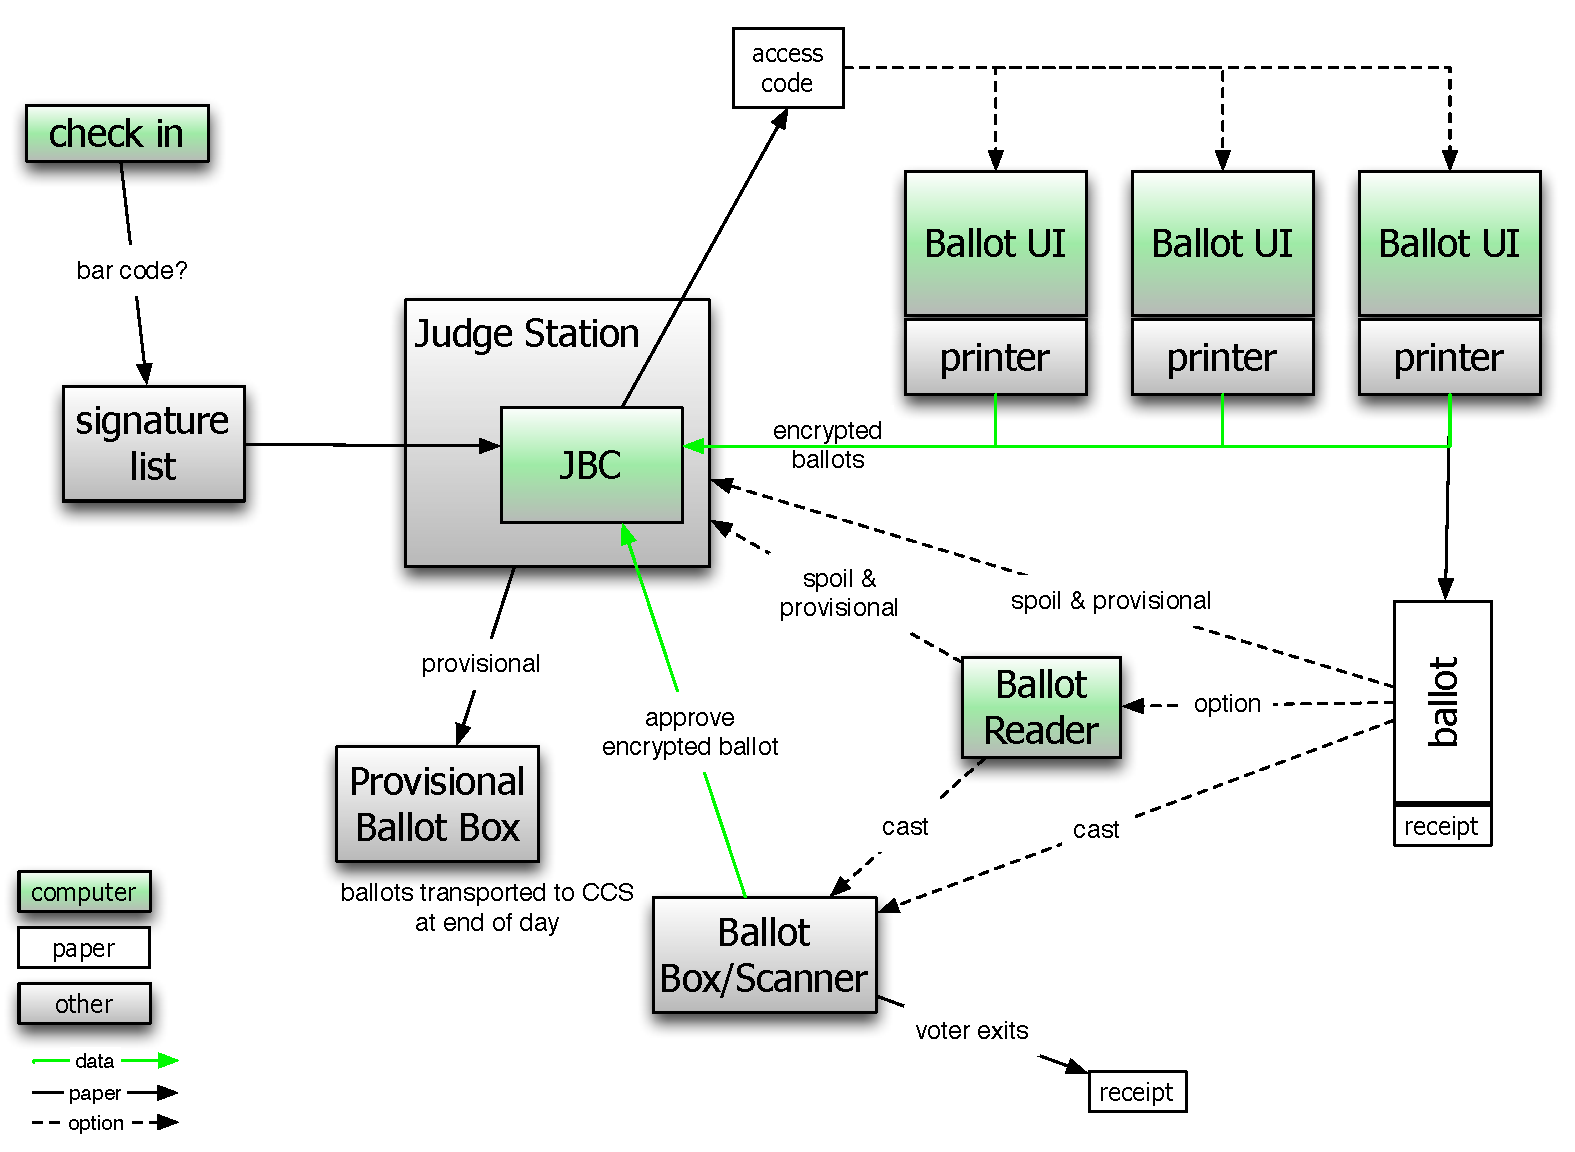
\includegraphics[width=6.5in]{TravisVote.pdf}
\caption{The design of the \projname system. Green objects are computers, white objects are paper records, and other objects are shaded in gray. Arrows display the flow of information; green for digital information, black for paper, and dashed lines indicate that the flow is contingent on voter choice.\label{fig:design}.}
\end{figure*}

Figure~\ref{fig:design} shows how \projname works from the perspective
of a voter going through the system. We note that the \projname voting system bears a resemblance to the Hart InterCivic eSlate system, or to VoteBox~\cite{sandler08votebox}, in that the voting machines are networked together, simplifying the movement of data. Like eSlate, we assume that a group of voting machines will share a common judge's station with a computer like Hart InterCivic's ``Judge Booth Controller'' (JBC) that manages everything. 

\begin{enumerate}
\item {\em Check-in (pollbook).}
The first step for the voter is to check-in with a poll worker. This is where voter registration is verified and the voter's precinct is identified so that the appropriate ballot style can be generated. The voter also signs a signature list. The voter will receive something to take with them to the JBC that identifies their ballot style; probably a piece of paper with a bar code on it. If the voter registration cannot be verified then this will identify them as requiring a provisional ballot.

\item {\em Receive token}
The voter takes the ballot style identifier to a poll worker at the Judge Booth Controller (JBC) which issues a token, again probably a piece of paper with a 5-digit code on it. (There will probably need to be a special alternative for ADA compliance as not all voters can see/handle paper.) This token authorizes the voter at a voting station and identifies his/her ballot style to the station. The token will also be flagged as provisional if that applies. The token has a limited life, so that the 5 digit sequence can be reused.

\item {\em Select machine}
The voter possibly queues at this point, and then selects from one of the available voting stations.

\item  {\em Enter token}
The first thing the voter does at the voting station is enter the information on their token. This causes the JBC to send the appropriate ballot style to the voting station and consumes the token.

\item {\em Make selections}
The voter makes selections on the GUI (for sighted voters) or auditory UI (for non-sighted voters). There is a review screen (or the auditory equivalent) so that the voter can confirm their selections before producing a paper record.

\item {\em Print}
When the voter has finished making selections, s/he tells the UI to print a paper record of their selections. This cryptographically commits the choices and sends their encrypted ballot to the JBC as well as printing a paper record, which includes not only a human-readable summary of the voter's selections but the encrypted ballot (as a bar code or something similar) and a human-readable crypto receipt (essentially a ballot ID number).

\item {\em Review printed record}
The voter may then review the printed record to confirm their selections. There will be at least one station available that can OCR the paper record and read it back to the voter for those who cannot read the paper record.

\item {\em Option: Cast, or challenge/spoil}
After review, the voter has two choices: either cast this ballot or spoil it. Spoiling the ballot may be because of an error (or change of heart) or because the voter wishes to challenge the crypto. The two procedures are described below. Note also that there is a special procedure for provisional ballots.

\begin{enumerate}
\item  {\em Cast Ballot}
If the voter wants to cast the ballot, s/he takes the paper record to the ballot box/scanner. The voter optionally removes the receipt and drops it into the box, where the bar code on the record is scanned. This is scan is communicated to the JBC, which then marks the vote as recorded (meaning it will be counted).

\item {\em Spoil Ballot}
If the paper record is to be spoiled, the voter returns to a poll worker at a JBC. The record will be placed in a special sleeve so that the poll worker cannot see the selections. The bar code on the record is scanned so that the JBC can record that the ballot is to be spoiled, which means that the decryption of the ballot will be published. The ballot will be stamped to indicate that it is a spoiled ballot. The voter may retain the paper record to check that the decryption matches the selections shown on the paper record. After the spoiled ballot is processed, then the voter is issued a new token.

\item {\em Provisional ballot}
In the case of a provisional ballot, the voter does not have the cast vs. spoil option, and must return the ballot to a poll worker, who places it into a provisional ballot box. The voter may retain the receipt to see if the ballot ends up being counted.
\end{enumerate}

\item {\em Optional: Voter checks crypto}
Using the receipt, after leaving the polling place, the ballots will be published. Cast votes are published in encrypted format, so the voter can check to make sure his/her vote is present and will be counted. In addition, any voter can check the tally of the cast votes. Spoiled votes are decrypted before publication so that the crypto can be challenged.
\end{enumerate}

<< sections 2.2 and 3 should go in here somewhere >>


%%% Local Variables: 
%%% mode: latex
%%% TeX-master: "star"
%%% End: 
